\section[碰撞]{\makebox[5em][s]{碰撞}}\label{sec:08.03}

所谓碰撞,包括相当广泛的一类物体间的相互作用过程。处
理碰撞问题,是动量守恒定律最重要的应用之一。

碰撞过程的基本特点如下:在碰撞之前,相碰的物体相距很
远,以致它们之间没有相互作用力,每个物体都处在自由运动的
状态,并且保持这种状态不变。当物体相互接近后,它们之间发
生作用,相互作用能够产生各种各样的结果。例如,可能使物体
结合在一起,也可能产生新的物体。在这种作用之后,物体又分离,
回到各自的自由运动状态不变。因此,碰撞所要讨论的是从碰前
的自由状态变到碰后自由状态的过程。显然,对于碰撞的中间过
程,是很难研究的。一方面,碰撞时物体之间的作用很强,要决
定力的具体形式,往往是十分复杂的;另一方面,我们很难直接
测量和记录碰撞时的现象。尤其是在原子实验中,对于电子和质
子相碰,记录它们碰撞时的情况,几乎是不可能的。但对碰撞前
和碰撞后进行测量是比较容易的。所以,在碰撞问题中,我们往
往是根据碰撞前和碰撞后的性质来研究相碰物体之间的相互作用
的性质。即通过碰撞的始末情况,我们能推测相互作用的某些性
质。例如,按照碰撞前与碰撞后物体的性质,可以将碰撞分成两
大类:弹性碰撞及非弹性碰撞。所谓弹性碰撞是指碰撞后的物体
仍然是原来的物体,而且这些物体的内部状态没有变化。碰撞后
的物体不同于碰撞前的,或者物体虽同但内部状态不同的碰撞都
属于非弹性碰撞。

在日常遇到的碰撞现象中,几乎都是不同程度的非弹性的。
因为碰撞往往伴随着使物体变热,即物体的动能部分地转化成
% 236.jpg
热能,这就改变了物体的内部运动状态。尽管如此,弹性碰撞概
念在物理中是非常重要的。因为,在原子、核子的碰撞现象中,
有许多是理想的弹性碰撞。由上述弹性与非弹性的分类原则,可
以断言:机械能守恒的碰撞,是弹性碰撞;机械能不守恒的碰撞,
\begin{wrapfigure}[10]{r}{17em}
  \centering
  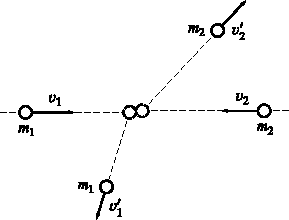
\includegraphics{figure/fig08.05}
  \caption{两质点的碰撞}
  \label{fig:08.05}
\end{wrapfigure}
是非弹性碰撞。因为后一情况必定伴随着其他形式能量的作用,也就
是伴随着改变物体的内部状态。

现在,我们来研究质量为$ m _ { 1 } $及$ m _ { 2 } $的两个
质点的弹性碰撞的一般性质。假设在碰撞前二质点的速度分别为
$ \vec{ v } _ { 1 } $和$ \vec{ v } _ { 2 } $,碰撞后分别是$ \vec{ v } ' _ { 1 } $和$ \vec{ v } ' _ { 1 } $
(图8.5)。根据动量守恒,有
\begin{equation}\label{eqn:08.03.01}
  m _ { 1 } \vec{ v } _ { 1 } + m _ { 2 } \vec{ v } _ { 2 } = m _ { 1 } \vec{ v } ' _ { 1 } + m _ { 2 } \vec{ v } ' _ { 2 }
\end{equation}
因为是弹性碰撞,故机械能守恒。由于碰撞前后两质点都处在没
有相互作用的自由运动状态,所以碰撞前后只有动能,根据机械
能守恒,总动能不变,即
\begin{equation}\label{eqn:08.03.02}
  \begin{split}
    & \frac { 1 } { 2 } m _ { 1 } v _ { 1 } ^ { 2 } + \frac { 1 } { 2 } m _ { 2 } v _ { 2 } ^ { 2 } \\
    = & \frac { 1 } { 2 } m _ { 1 } { v ' _ { 1 } } ^ { 2 } + \frac { 1 } { 2 } m _ { 2 } { v ' _ { 2 } } ^ { 2 }
  \end{split}
\end{equation}
式\eqref{eqn:08.03.01}、\eqref{eqn:08.03.02}就是弹性碰撞
所应遵循的两个一般的关系。

式\eqref{eqn:08.03.01}、\eqref{eqn:08.03.02}没有涉及碰撞
物体间相互作用力的具体性质。这表明即使我们对它们之间的相互作
用力的细节不清楚,也可以得到一些碰撞所必须遵守的一般关系。这个
例子再次说明了守恒定律在讨论力学问题时的重要性。当然,如果我们
想知道
% 237.jpg
碰撞的细节,则必须弄清作用力的具体情况。

在加速器的粒子碰撞实验中,靶上的粒子是不动的,因此有
$ \vec { v } _ { 1 } \ne 0 $,$ \vec { v } _ { 2 } = 0 $。
我们首先讨论一种简单的情况。假定所有的速度方向都是平行或反平
行,即化为一维问题,这时式\eqref{eqn:08.03.01}、
\eqref{eqn:08.03.02}可写为
\begin{align}
  m _ { 1 } v _ { 1 }               & = m _ { 1 } v ' _ { 1 } + m _ { 2 } v ' _ { 2 } \label{eqn:08.03.03}                         \\
  m _ { 1 } { v ' _ { 1 } } ^ { 2 } & = m _ { 1 } { v ' _ { 1 } } ^ { 2 } + m _ { 2 } { v ' _ { 2 } } ^ { 2 } \label{eqn:08.03.04}
\end{align}
上两式可改写为
\begin{align}
  m _ { 2 } v ' _ { 2 }             & = m _ { 1 } \left( v _ { 1 } - v ' _ { 1 } \right) \label{eqn:08.03.05}                     \\
  m _ { 2 } { v ' _ { 2 } } ^ { 2 } & = m _ { 1 } \left( v _ { 1 } ^ { 2 } - { v ' _ { 1 } } ^ { 2 } \right) \label{eqn:08.03.06}
\end{align}
将两式相除,得到
\begin{equation*}
  v _ { 2 } = v _ { 1 } + v ' _ { 1 }
\end{equation*}
再与式\eqref{eqn:08.03.05}联立解之,发现
\begin{equation}\label{eqn:08.03.07}
  \begin{split}
    v ' _ { 1 } & = \frac { m _ { 1 } - m _ { 2 } } { m _ { 1 } + m _ { 2 } } v _ { 1 } \\
    v ' _ { 2 } & = \frac { 2 m _ { 1 } } { m _ { 1 } + m _ { 2 } } v _ { 1 }
  \end{split}
\end{equation}
由解式\eqref{eqn:08.03.07},可以得出一些有用的结论:
当$ m _ { 1 } > m _ { 2 } $,$ v ' _ { 1 } > 0 $,
即入射粒子碰撞后仍向前运动;
当$ m _ { 1 } < m _ { 2 } $,$ v ' _ { 1 } < 0 $,
即入射粒子碰撞后向反向运动了;
若$ m _ { 1 } = m _ { 2 } $,则$ v ' _ { 1 } = 0 $,
而$ v ' _ { 2 } = v _ { 1 } $,这相当于两个粒子的速度
相互交换了。

现在讨论另一种简单情况,即相碰撞的两个粒子的质量是一
样的($ m _ { 1 } = m _ { 2 } $),且$ \vec { v } _ { 2 } = 0 $,
但速度方向不一定是平行或反平行。
这时,式\eqref{eqn:08.03.01}、\eqref{eqn:08.03.02}成为
\begin{align}
  \vec { v } _ { 1 } & = \vec { v } ' _ { 1 } + \vec { v } ' _ { 2 } \label{eqn:08.03.08}       \\
  v _ 1 ^ { 2 }      & = { v ' _ { 1 } } ^ { 2 } + { v ' _ { 2 } } ^ { 2 } \label{eqn:08.03.09}
\end{align}
式\eqref{eqn:08.03.08}表明,三个矢量$ \vec { v } _ { 1 } $,$ \vec { v } ' _ { 1 } $,$ \vec { v } ' _ { 2 } $,构成一个三角形;而从式
% 238.jpg
\eqref{eqn:08.03.09}可以知道,这个三角形必定是以
$ \vec { v } _ { 1 } $为斜边的直角三角形
(图\ref{fig:08.06}),因而$ \vec { v } ' _ { 1 } $和$ \vec { v } ' _ { 2 } $必定互相垂直,即在碰撞后,两粒子的运动
方向一定是相互垂直的。由此,我们得到一个非常有用的图形,
称为散射圆(图\ref{fig:08.07})。圆的直径是$ v _ { 1 } $,由于$ \vec { v } ' _ { 1 } \perp \vec { v } ' _ 2 $,所以,直角
\begin{figure}[h]
  \begin{minipage}[b]{0.5\linewidth}
    \centering
    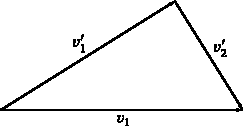
\includegraphics{figure/fig08.06}
    \caption{碰撞速度之间的关系}
    \label{fig:08.06}
  \end{minipage}
  \begin{minipage}[b]{0.5\linewidth}
    \centering
    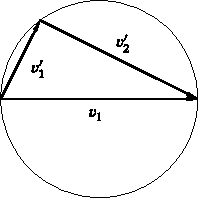
\includegraphics{figure/fig08.07}
    \caption{散射圆}
    \label{fig:08.07}
  \end{minipage}
\end{figure}
三角形的顶端一定在圆周上。这样,如果测得了入射粒子碰撞后
的运动方向,从图上可以立即求得靶中被撞出的粒子的速度的大
小和方向。

这个结果在实验中很有实用价值。譬如,在研究质子与质子
\begin{wrapfigure}[7]{r}{15em}
  \centering
  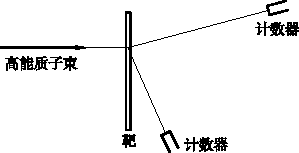
\includegraphics{figure/fig08.08}
  \caption{测量质子-质子弹性散射}
  \label{fig:08.08}
\end{wrapfigure}
弹性碰撞的实验中,我们知道,高能质子打在靶上,会
撞出多种粒子,它们都是非弹性碰撞。我们如何才能专
门测得质子与质子的弹性碰撞呢?根据上述分析,如果
把两个测量质子的计数器放
在相互垂直的位置(图\ref{fig:08.08}),并且测量符合散射圆的质子,则我们
测得的就是弹性碰撞的事件。

对于质量不等的粒子间的碰撞,我们也可以求得类似的散射
图,用以指导我们的实验。
